\documentclass[11pt]{article}
\usepackage[margin=1in]{geometry}
\usepackage{amsmath,amssymb}
\usepackage{enumerate}
\usepackage{array}
\usepackage{xcolor}
\usepackage{tikz}
\setlength{\parindent}{0pt}
\setlength{\parskip}{4pt}

\newcommand{\question}[1]{\par\smallskip\noindent\colorbox{black!6}{\parbox{\dimexpr\linewidth-2\fboxsep}{\itshape #1}}\par\smallskip}

\title{Problem set 3 \\ \large Solution Key}
\author{Econ 5030}
\date{}

\begin{document}
\maketitle

The question text is reproduced in the grey boxes. Everything after a box is the answer.

%%%%%%%%%%%%%%%%%%%%%%%%%%%%%%%%%%%%%%%%%%%%%%%%%%%%%%%%%%%%%%%%%%%%%%%
\section{Basic Cournot duopoly}

\question{Let begin by considering a Cournot duopoly. Each firm $i$ has the cost function $C(q_i)=cq_i^2/2$, where $c>0$. Market inverse $P(Q)=200-Q$.}

\question{\textbf{1.a} Write the profit of the arbitrary firm $i$.}

With $Q=q_i+q_j$,
\[
\pi_i(q_i,q_j)=(200-q_i-q_j)\,q_i-\frac{c}{2}q_i^2 .
\]

\question{\textbf{1.b} Find the best response function for firm $i$ and graph it on the $q_i\times q_j$ plane.}

$\pi_i$ is strictly concave in $q_i$ ($\partial^2\pi_i/\partial q_i^2=-(2+c)<0$), so the first-order condition is sufficient:
\[
\frac{\partial\pi_i}{\partial q_i}=200-2q_i-q_j-cq_i=0
\quad\Longrightarrow\quad
BR_i(q_j)=\max\Big\{\frac{200-q_j}{2+c},\,0\Big\}.
\]
It is a downward-sloping line with $q_i$-intercept $200/(2+c)$ (the monopoly output) and $q_j$-intercept $200$ (the competitive output, where price would hit zero). Quantities are strategic substitutes: the slope is $-1/(2+c)$.

\begin{center}
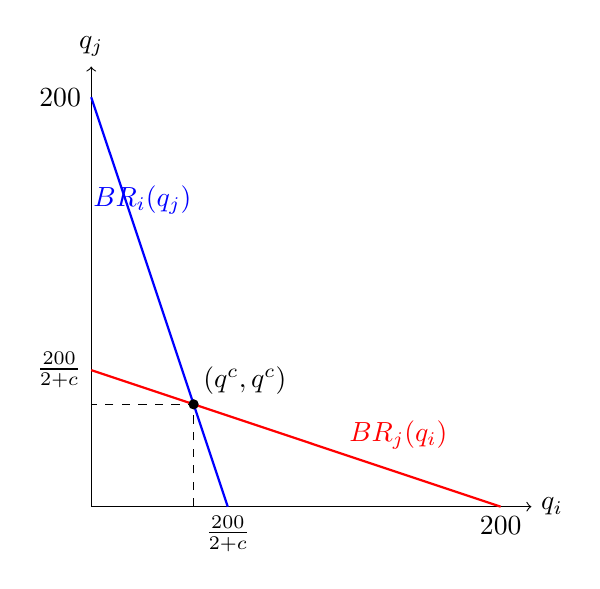
\begin{tikzpicture}[scale=0.026]
  \draw[->] (0,0) -- (215,0) node[right] {$q_i$};
  \draw[->] (0,0) -- (0,215) node[above] {$q_j$};
  % c = 1 used for the picture: intercepts 200/3
  \draw[thick,blue] (66.7,0) -- (0,200) node[left,black] {$200$};
  \draw[thick,red] (0,66.7) -- (200,0) node[below,black] {$200$};
  \node[below] at (66.7,0) {$\frac{200}{2+c}$};
  \node[left] at (0,66.7) {$\frac{200}{2+c}$};
  \fill (50,50) circle (2.5);
  \draw[dashed] (50,0) -- (50,50) -- (0,50);
  \node[above right] at (50,50) {$(q^c,q^c)$};
  \node[blue] at (25,150) {$BR_i(q_j)$};
  \node[red] at (150,35) {$BR_j(q_i)$};
\end{tikzpicture}
\end{center}

\question{\textbf{1.c} Find the Cournot equilibrium quantity $q^c$ and market price $p^c=P(2q^c)$.}

The game is symmetric, so set $q_i=q_j=q^c$ in the best response: $(2+c)q^c=200-q^c$, so
\[
q^c=\frac{200}{3+c},\qquad Q^c=\frac{400}{3+c},\qquad
p^c=200-\frac{400}{3+c}=\frac{200(1+c)}{3+c}.
\]
(The equilibrium is unique: the two best-response lines have slopes $-1/(2+c)$ and $-(2+c)$, so they cross once.)

\question{\textbf{1.d} Graph the market outcome on the $p\times Q$ plane.}

Each firm's marginal cost is $MC_i=cq_i$, so firm supply is $q_i=p/c$ and industry supply (the sum of marginal cost curves) is $Q=2p/c$, i.e.\ $p=cQ/2$. The efficient point is where demand meets this supply curve:
\[
200-Q=\tfrac{c}{2}Q\ \Longrightarrow\ Q^*=\frac{400}{2+c},\qquad p^*=\frac{200c}{2+c}.
\]
Cournot output $Q^c<Q^*$ and price $p^c>p^*$.

\begin{center}
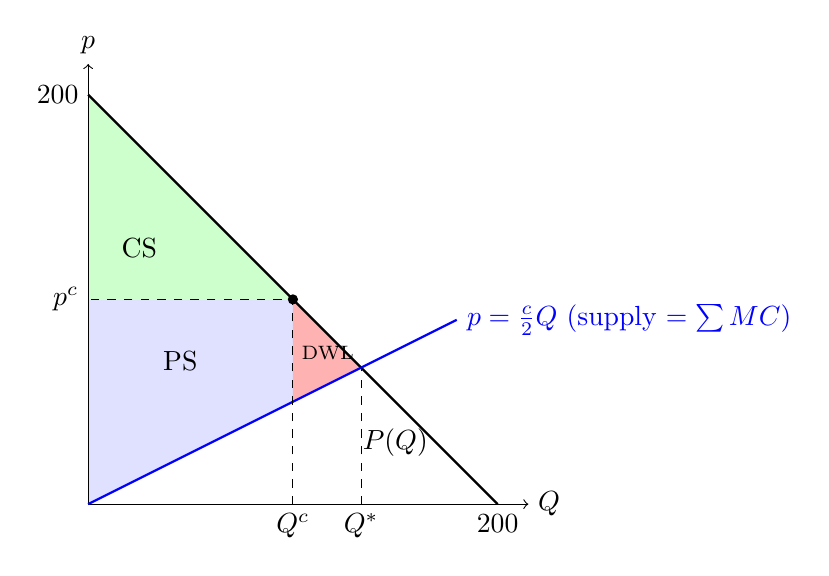
\begin{tikzpicture}[scale=0.026]
  % picture drawn for c = 1: Q^c = 100, p^c = 100, Q* = 133.3, p* = 66.7, MC at Q^c = 50
  \fill[green!20] (0,200) -- (0,100) -- (100,100) -- cycle;
  \fill[blue!12] (0,0) -- (0,100) -- (100,100) -- (100,50) -- cycle;
  \fill[red!30] (100,100) -- (133.3,66.7) -- (100,50) -- cycle;
  \draw[->] (0,0) -- (215,0) node[right] {$Q$};
  \draw[->] (0,0) -- (0,215) node[above] {$p$};
  \draw[thick] (0,200) -- (200,0) node[below] {$200$};
  \node[left] at (0,200) {$200$};
  \draw[thick,blue] (0,0) -- (180,90) node[right] {$p=\tfrac{c}{2}Q$ (supply $=\sum MC$)};
  \node at (150,30) {$P(Q)$};
  \draw[dashed] (100,0) node[below] {$Q^c$} -- (100,100) -- (0,100) node[left] {$p^c$};
  \draw[dashed] (133.3,0) node[below] {$Q^*$} -- (133.3,66.7);
  \fill (100,100) circle (2.5);
  \node at (25,125) {CS};
  \node at (45,70) {PS};
  \node at (117,74) {\scriptsize DWL};
\end{tikzpicture}
\end{center}
(The picture uses $c=1$ for scale. CS is the triangle above $p^c$, PS is the area between $p^c$ and the supply curve up to $Q^c$, and the deadweight loss is the triangle between demand and supply from $Q^c$ to $Q^*$.)

\question{\textbf{1.e} Find an expression for the each firm's profits, the Consumer Surplus (CS), Total Surplus (TS) and Dead weight Loss (DWL).}

\emph{Profit.} $\pi^c=p^cq^c-\tfrac{c}{2}(q^c)^2=q^c\big(p^c-\tfrac{c}{2}q^c\big)
=\frac{200}{3+c}\cdot\frac{200(1+c)-100c}{3+c}$, so
\[
\pi^c=\frac{20000(2+c)}{(3+c)^2}.
\]
\emph{Consumer surplus.} Demand has slope $-1$, so $CS=\tfrac12(200-p^c)Q^c=\tfrac12(Q^c)^2$:
\[
CS=\frac{80000}{(3+c)^2}.
\]
\emph{Total surplus.} $TS=CS+2\pi^c=\dfrac{80000+40000(2+c)}{(3+c)^2}$, so
\[
TS=\frac{40000(4+c)}{(3+c)^2}.
\]
\emph{Deadweight loss.} The maximum total surplus is the triangle between demand and supply from $0$ to $Q^*$: $TS^*=\tfrac12\cdot200\cdot Q^*=\dfrac{40000}{2+c}$. Then
\[
DWL=TS^*-TS=40000\,\frac{(3+c)^2-(4+c)(2+c)}{(2+c)(3+c)^2}=\frac{40000}{(2+c)(3+c)^2}.
\]
\emph{Check} ($c=2$, i.e.\ $C=q^2$): $q^c=40$, $p^c=120$, $\pi^c=3200$, $CS=3200$, $TS=9600$, $TS^*=10000$, $DWL=400$.

%%%%%%%%%%%%%%%%%%%%%%%%%%%%%%%%%%%%%%%%%%%%%%%%%%%%%%%%%%%%%%%%%%%%%%%
\section{Basic Cournot oligopoly}

\question{Let now consider a Cournot oligopoly with $n$ firms. Each firm $i$ has the cost function $C(q_i)=cq_i^2/2$, where $c>0$. Market inverse $P(Q)=200-Q$.}

\question{\textbf{2.a} Write the profit of the arbitrary firm $i$.}

With $Q_{-i}=\sum_{j\ne i}q_j$,
\[
\pi_i(q_i,Q_{-i})=(200-q_i-Q_{-i})\,q_i-\frac{c}{2}q_i^2 .
\]

\question{\textbf{2.b} Find the best response function for firm $i$ and graph it on the $q_i\times Q_{-i}$ plane.}

Same algebra as 1.b with $q_j$ replaced by $Q_{-i}$ (still strictly concave):
\[
200-2q_i-Q_{-i}-cq_i=0\quad\Longrightarrow\quad BR_i(Q_{-i})=\max\Big\{\frac{200-Q_{-i}}{2+c},\,0\Big\}.
\]
Firm $i$ cares only about the total output of its rivals, not how it is split.

\begin{center}
\begin{tikzpicture}[scale=0.026]
  \draw[->] (0,0) -- (215,0) node[right] {$q_i$};
  \draw[->] (0,0) -- (0,215) node[above] {$Q_{-i}$};
  \draw[thick,blue] (66.7,0) -- (0,200) node[left,black] {$200$};
  \node[below] at (66.7,0) {$\frac{200}{2+c}$};
  \draw[dashed,gray] (0,0) -- (80,160) node[above right,black] {\small $Q_{-i}=(n-1)q_i$};
  \fill (40,80) circle (2.5);
  \node[right] at (42,78) {\small equilibrium};
  \node[blue] at (32,170) {$BR_i(Q_{-i})$};
\end{tikzpicture}
\end{center}
In a symmetric equilibrium the best-response line meets the ray $Q_{-i}=(n-1)q_i$. (Drawn for $c=1$, $n=3$.)

\question{\textbf{2.c} Find the Cournot equilibrium quantity $q^c$ and market price $p^c=P(nq^c)$.}

In the symmetric equilibrium $Q_{-i}=(n-1)q^c$, so $(2+c)q^c=200-(n-1)q^c$:
\[
q^c=\frac{200}{n+1+c},\qquad Q^c=\frac{200n}{n+1+c},\qquad p^c=200-Q^c=\frac{200(1+c)}{n+1+c}.
\]
With $n=2$ this is 1.c. As $n\to\infty$: $q^c\to0$, $Q^c\to200$ and $p^c\to0$.

\question{\textbf{2.d} Graph the market outcome on the $p\times Q$ plane.}

Industry supply is now $Q=np/c$, i.e.\ $p=\tfrac{c}{n}Q$, which gets flatter as $n$ grows. The efficient point is
\[
200-Q=\tfrac{c}{n}Q\ \Longrightarrow\ Q^*=\frac{200n}{n+c},\qquad p^*=\frac{200c}{n+c}.
\]

\begin{center}
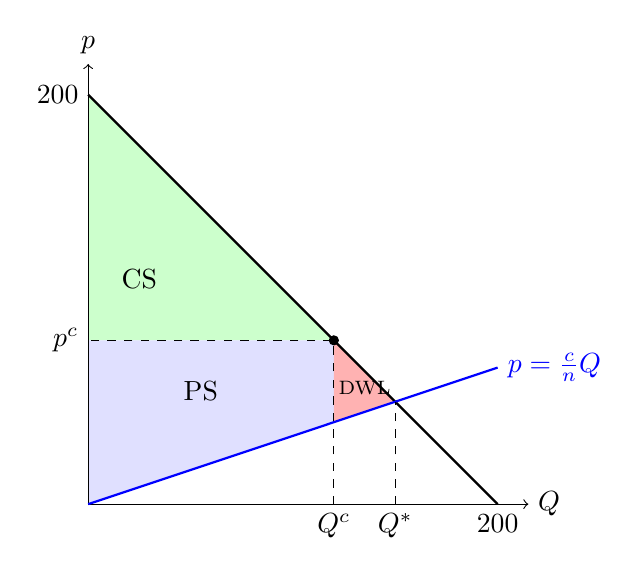
\begin{tikzpicture}[scale=0.026]
  % drawn for c = 1, n = 3: Q^c = 120, p^c = 80, Q* = 150, p* = 50, MC at Q^c = 40
  \fill[green!20] (0,200) -- (0,80) -- (120,80) -- cycle;
  \fill[blue!12] (0,0) -- (0,80) -- (120,80) -- (120,40) -- cycle;
  \fill[red!30] (120,80) -- (150,50) -- (120,40) -- cycle;
  \draw[->] (0,0) -- (215,0) node[right] {$Q$};
  \draw[->] (0,0) -- (0,215) node[above] {$p$};
  \draw[thick] (0,200) -- (200,0) node[below] {$200$};
  \node[left] at (0,200) {$200$};
  \draw[thick,blue] (0,0) -- (200,66.7) node[right] {$p=\tfrac{c}{n}Q$};
  \draw[dashed] (120,0) node[below] {$Q^c$} -- (120,80) -- (0,80) node[left] {$p^c$};
  \draw[dashed] (150,0) node[below] {$Q^*$} -- (150,50);
  \fill (120,80) circle (2.5);
  \node at (25,110) {CS};
  \node at (55,55) {PS};
  \node at (135,57) {\scriptsize DWL};
\end{tikzpicture}
\end{center}
Same picture as 1.d: CS above $p^c$, PS between $p^c$ and the supply curve, DWL the triangle from $Q^c$ to $Q^*$. As $n$ rises, $Q^c$ moves toward $Q^*$ and the triangle shrinks. (Drawn for $c=1$, $n=3$.)

\question{\textbf{2.e} Find an expression for the each firm's profits, the Consumer Surplus (CS), Total Surplus (TS) and Dead weight Loss (DWL).}

\emph{Profit.} $\pi^c=q^c\big(p^c-\tfrac{c}{2}q^c\big)=\dfrac{200}{n+1+c}\cdot\dfrac{200(1+c)-100c}{n+1+c}$, so
\[
\pi^c=\frac{20000(2+c)}{(n+1+c)^2}.
\]
\emph{Consumer surplus.} $CS=\tfrac12(Q^c)^2=\dfrac{20000\,n^2}{(n+1+c)^2}$.

\emph{Total surplus.} $TS=CS+n\pi^c=\dfrac{20000\,n^2+20000\,n(2+c)}{(n+1+c)^2}=\dfrac{20000\,n(n+2+c)}{(n+1+c)^2}$.

\emph{Deadweight loss.} $TS^*=\tfrac12\cdot200\cdot Q^*=\dfrac{20000\,n}{n+c}$. Let $m=n+c$. Then $(m+1)^2-m(m+2)=1$, so
\[
DWL=20000\,n\Big[\frac{1}{n+c}-\frac{n+2+c}{(n+1+c)^2}\Big]=\frac{20000\,n}{(n+c)(n+1+c)^2}.
\]
\emph{Checks.} With $n=2$, every formula reduces to 1.e. As $n\to\infty$, $DWL\sim20000/n^2\to0$ and $\pi^c\to0$: more competition moves the market toward the efficient outcome. Example ($c=1$, $n=4$): $q^c=33.3$, $p^c=66.7$, $\pi^c=1666.7$, $DWL=444.4$.

%%%%%%%%%%%%%%%%%%%%%%%%%%%%%%%%%%%%%%%%%%%%%%%%%%%%%%%%%%%%%%%%%%%%%%%
\section{Cournot with product differentiation}

\question{Take the inverse demand system:
\[
P_1(q_1,q_2)=18-q_1-\gamma q_2,\qquad P_2(q_2,q_1)=18-q_2-\gamma q_1 .
\]
Assume both firms have NO COST of production. Now let us look at the Cournot solution for general $\gamma$ between zero an one.}

The parts are printed as 2.a--2.d in the problem set. They are labelled 3.a--3.d here.

\question{\textbf{3.a} Write out each firm's profit function and label them $\Pi_1(\gamma)$ and $\Pi_2(\gamma)$.}

\[
\Pi_1(\gamma)=(18-q_1-\gamma q_2)\,q_1,\qquad \Pi_2(\gamma)=(18-q_2-\gamma q_1)\,q_2 .
\]

\question{\textbf{3.b} Find each firm's best response function by solving $\dfrac{\partial\Pi_1(\gamma)}{\partial q_1}=0$ for $q_1^\gamma(q_2)$ and $\dfrac{\partial\Pi_2(\gamma_2,\gamma_1)}{\partial q_2}=0$ for $q_2^\gamma(q_1)$.}

Each profit is strictly concave in own output (second derivative $-2$).
\[
\frac{\partial\Pi_1}{\partial q_1}=18-2q_1-\gamma q_2=0\ \Longrightarrow\ q_1^\gamma(q_2)=\frac{18-\gamma q_2}{2},
\]
\[
\frac{\partial\Pi_2}{\partial q_2}=18-2q_2-\gamma q_1=0\ \Longrightarrow\ q_2^\gamma(q_1)=\frac{18-\gamma q_1}{2}.
\]
The parameter $\gamma$ measures how much the rival's output lowers my price, i.e.\ how close substitutes the goods are. $\gamma=0$: independent goods (two monopolies). $\gamma=1$: perfect substitutes (homogeneous Cournot).

\question{\textbf{3.c} Graph the best response functions of the firms' on $q_1\times q_2$ space.}

$q_1^\gamma(q_2)$ runs from $(9,0)$ to $(0,18/\gamma)$; $q_2^\gamma(q_1)$ runs from $(0,9)$ to $(18/\gamma,0)$. A larger $\gamma$ makes each line steeper relative to its own axis and pulls the crossing toward the origin.

\begin{center}
\begin{tikzpicture}[scale=0.3]
  % drawn for gamma = 1/2: intercepts 9 and 36, crossing at 7.2
  \draw[->] (0,0) -- (21,0) node[right] {$q_1$};
  \draw[->] (0,0) -- (0,21) node[above] {$q_2$};
  \draw[thick,blue] (9,0) -- (4,20) node[right] {$q_1^\gamma(q_2)\ \uparrow (0,\frac{18}{\gamma})$};
  \draw[thick,red] (0,9) -- (20,4) node[right] {$q_2^\gamma(q_1)\ \to(\frac{18}{\gamma},0)$};
  \node[below] at (9,0) {$9$};
  \node[left] at (0,9) {$9$};
  \fill (7.2,7.2) circle (0.25);
  \draw[dashed] (7.2,0) node[below] {\scriptsize $\frac{18}{2+\gamma}$} -- (7.2,7.2) -- (0,7.2);
\end{tikzpicture}
\end{center}
(Drawn for $\gamma=\tfrac12$, where the $18/\gamma=36$ intercepts are off the picture.)

\question{\textbf{3.d} Find the equilibrium quantities and prices and label them $q_1(\gamma)$, $p_1(\gamma)$ and $q_2(\gamma)$, $p_2(\gamma)$.}

By symmetry $q_1=q_2=q$: $2q=18-\gamma q$, so
\[
q_1(\gamma)=q_2(\gamma)=\frac{18}{2+\gamma},\qquad
p_1(\gamma)=p_2(\gamma)=18-(1+\gamma)\frac{18}{2+\gamma}=\frac{18}{2+\gamma},
\qquad \Pi_i=\frac{324}{(2+\gamma)^2}.
\]
(Direct check without imposing symmetry: subtracting the two first-order conditions gives $(2-\gamma)(q_1-q_2)=0$, so $q_1=q_2$ since $\gamma<2$.)

Price, quantity and profit all fall as $\gamma$ rises. At $\gamma=0$: $q=p=9$, $\Pi=81$ (each firm is a monopolist). At $\gamma=1$: $q=p=6$, $\Pi=36$ (homogeneous Cournot). Product differentiation softens competition.

%%%%%%%%%%%%%%%%%%%%%%%%%%%%%%%%%%%%%%%%%%%%%%%%%%%%%%%%%%%%%%%%%%%%%%%
\section{Price competition}

\question{Suppose that thre are 2 firms in a Bertrand oligopoly with homogenous products. Each firm $i$ has th cost of production $c(q_i)=q_i^2/2$. The industry demand function is the rectangle
\[
D(p)=\begin{cases}0 & \text{if } p>10\\ 10 & \text{if } p\le 10\end{cases}
\]
The if firms price the same then demand is split evenly. Each firm $i$ has th cost of production $c(q_i)=q_i^2/2$. Based on this cost structure a firm will never supply more than their supply function $s(p_i)=p_i$. using this fact we can construct residual demand and firm profit. Firm profit is the piecewise function for prices in the interval $[0,10]$ (I have done all the work for you here):
\[
\pi_i(p_i,p_j)=\begin{cases}
p_i\min\{p_i,10-p_j\}-\big(\min\{p_i,10-p_j\}\big)^2/2 & p_i>p_j\\
p_i5-12.5 & p_i=p_j>5\\
p_i^2/2 & p_i=p_j\le5\\
p_i^2/2 & p_i<p_j
\end{cases}
\]}

Two facts used throughout:
\begin{itemize}
\item[(A)] \emph{Low price:} $p_i<p_j$ gives $p_i^2/2$, strictly increasing in $p_i$.
\item[(B)] \emph{High price:} for $p_i>p_j$, profit is increasing in $p_i$ on both pieces of the min and continuous where they meet, so the best high price is $p_i=10$. There the firm sells the residual $10-p_j$:
\[
\pi_i(10,p_j)=10(10-p_j)-\tfrac12(10-p_j)^2=\frac{(10-p_j)(10+p_j)}{2}=\frac{100-p_j^2}{2}.
\]
\end{itemize}

\question{\textbf{1.} Because for most prices $p_j$ the best response is not well-defined, instead find the argument of the supremum of the profit responding to the other firm's price. Formally find
\[
\phi(p_j)=\arg\sup_{p_i\in[0,10]}\pi_i(p_i,p_j)
\]}

Compare the three options against $p_j$:
\begin{itemize}
\item Undercut ($p_i<p_j$): by (A) the supremum is $p_j^2/2$, approached as $p_i\uparrow p_j$ but not attained.
\item Match ($p_i=p_j$): $p_j^2/2$ if $p_j\le5$; $5p_j-12.5$ if $p_j>5$. Since $p_j^2/2-(5p_j-12.5)=\tfrac12(p_j-5)^2>0$ for $p_j>5$, matching is never better than undercutting.
\item Go high ($p_i=10$): $(100-p_j^2)/2$ by (B), available when $p_j<10$.
\end{itemize}
Going high beats undercutting iff $100-p_j^2>p_j^2$, i.e.\ $p_j<\sqrt{50}=5\sqrt2\approx7.07$. Therefore
\[
\phi(p_j)=\begin{cases}
\{10\} & 0\le p_j\le5\sqrt2 \quad(\text{at } p_j=5\sqrt2 \text{ both give } 25)\\[2pt]
p_j^- \ (\text{just below } p_j) & 5\sqrt2<p_j\le10
\end{cases}
\]
where $p_j^-$ means the supremum $p_j^2/2$ is approached by $p_j-\varepsilon$, $\varepsilon\downarrow0$, and is not attained. This is why a best response does not exist for $p_j>5\sqrt2$.

\question{\textbf{2.} Make a formal argument that symmetric prices cannot be a pure strategy Nash equilibrium.}

Suppose $p_1=p_2=p$.
\begin{itemize}
\item If $p\le5$: each earns $p^2/2\le12.5$. Deviating to $10$ gives $(100-p^2)/2\ge37.5>p^2/2$. Profitable.
\item If $5<p\le10$: each earns $5p-12.5$. Undercutting to $p-\varepsilon$ gives $(p-\varepsilon)^2/2\to p^2/2$, and $p^2/2-(5p-12.5)=\tfrac12(p-5)^2>0$, so a small enough $\varepsilon$ is profitable.
\end{itemize}
Every symmetric profile has a profitable deviation, so none is a Nash equilibrium. (Intuition: below 5 the capacity-like supply limit leaves residual demand worth serving at the top price; above 5 a firm wants its whole supply $p$ rather than half the market, $5$.)

\question{\textbf{3.} Make a formal argument that asymmetric prices cannot be a pure strategy Nash equilibrium.}

Suppose $p_j<p_i$. The low-priced firm $j$ earns $p_j^2/2$ by (A). Any $p_j'\in(p_j,p_i)$ still undercuts $i$, so $j$ still sells its full supply, and it earns $p_j'^2/2>p_j^2/2$. So $j$ has a profitable deviation and $(p_i,p_j)$ is not a Nash equilibrium. Combined with 2, there is no pure strategy Nash equilibrium.

\question{\textbf{4.} Use your result from 1 to find the bound of best response prices.}

From 1, every best (supremum) response to a pure price is either $10$ or just below some $p_j>5\sqrt2$. So best-response prices lie in
\[
[\,5\sqrt2,\ 10\,]\approx[7.07,\ 10].
\]
The upper bound $\bar p=10$ is the price a firm uses when it accepts being the high-priced firm: once it is the high firm, it should charge the most it can for the residual demand. Prices below $5\sqrt2$ are never a best response to a pure price, since against $p_j<5\sqrt2$ the firm would rather jump to 10.

\question{\textbf{5.} Solve for the mixed strategy equilibrium using pricing bounds using the answer to 1.}

Look for a symmetric equilibrium in which each firm draws its price from a CDF $F$ with support $[\underline p,10]$.

\emph{No atoms.} An atom at a price $p>5$ cannot occur: the rival would gain by moving that mass to just below $p$, because tying earns $5p-12.5<p^2/2$. In particular there is no atom at $10$, and none at $\underline p$.

\emph{Upper bound} $\bar p=10$. By (B), whenever a firm is the high-priced firm it is best off at 10, so the top of the support is $10$.

\emph{Lower bound.} At $\underline p$ a firm is the low-priced firm with probability 1, so its equilibrium payoff is $k=\underline p^{\,2}/2$. At $10$ it is the high-priced firm with probability 1, so $k=E\big[(100-X^2)/2\big]$ where $X\sim F$ is the rival's price. Indifference between the two ends gives
\[
\frac{\underline p^{\,2}}{2}=50-\frac{E[X^2]}{2}\quad\Longleftrightarrow\quad E[X^2]=100-\underline p^{\,2}.
\]
Note: $\underline p$ cannot equal the pure-strategy bound $5\sqrt2$ from 4. If it did, $E[X^2]=50=\underline p^{\,2}$, which would put all of $F$'s mass at $\underline p$, and that contradicts no atoms. Against a \emph{mixed} rival, prices somewhat below $5\sqrt2$ become worthwhile. So the bound is pinned down together with $F$ (part 6): $\underline p\approx6.60$.

\question{\textbf{6.} Solve for the Nash Equilibrium Mixed strategies.}

For $p\in[\underline p,10]$ and a rival price $x<p$, the high firm sells $\min\{p,10-x\}=10-x$ (since $10-x\le10-\underline p<\underline p\le p$). Expected profit from $p$ is
\[
\pi(p)=\int_{\underline p}^{p}\Big[p(10-x)-\tfrac12(10-x)^2\Big]dF(x)+\big(1-F(p)\big)\frac{p^2}{2}=k \quad\text{for all } p\in[\underline p,10].
\]
Differentiate once. The terms with $f(p)$ combine to $\big[p(10-p)-\tfrac12(10-p)^2-\tfrac12p^2\big]f(p)=-2(p-5)^2f(p)$, so
\[
\int_{\underline p}^{p}(10-x)\,dF(x)+p\big(1-F(p)\big)-2(p-5)^2f(p)=0 .
\]
Differentiate again and write $S=1-F$, $t=p-5$:
\[
2t^2S''+6tS'+S=0 .
\]
This is an Euler equation. Trying $S=t^r$ gives $2r^2+4r+1=0$, so $r=-1\pm\tfrac{1}{\sqrt2}$. Imposing $S=0$ at $p=10$ ($t=5$) gives
\[
F(p)=1-C\Big[5^{\sqrt2}(p-5)^{-1-\frac{1}{\sqrt2}}-(p-5)^{-1+\frac{1}{\sqrt2}}\Big],\qquad \underline p\le p\le10 .
\]
The remaining two conditions are $F(\underline p)=0$ and the first-derivative equation at $p=\underline p$, i.e.\ $\underline p=2(\underline p-5)^2f(\underline p)$. Solving them numerically:
\[
\underline p\approx6.602,\qquad C\approx0.2869 .
\]
\begin{center}
\begin{tabular}{c|cccccc}
$p$ & $6.60$ & $7$ & $7.5$ & $8$ & $9$ & $10$\\ \hline
$F(p)$ & $0$ & $0.378$ & $0.635$ & $0.780$ & $0.929$ & $1$
\end{tabular}
\end{center}
The density is positive on the whole support, the mean price is about $7.47$, and $E[X^2]\approx56.41=100-\underline p^{\,2}$, which checks the condition from 5. I also checked numerically that $\pi(p)$ is constant ($\approx21.79$) at every price in $[\underline p,10]$. Below $\underline p$, $\pi(p)=p^2/2<k$, so no price outside the support pays more.

The Nash equilibrium is: each firm independently draws its price from $F$ on $[6.60,10]$.

\question{\textbf{7.} Calculate the Nash equilibrium expected profits.}

\[
E[\pi_i]=k=\frac{\underline p^{\,2}}{2}\approx\frac{6.602^2}{2}\approx21.8\ \text{per firm}.
\]
For comparison: two price-takers at $p=5$ would each sell $5$ and earn $12.5$. Joint profit maximization (both at $10$, each selling 5) would give each $37.5$. Mixed pricing lands between the two.

\end{document}
